\Aufgabe[ACTL \& LTL\hfill\textbf{(2 Points)}]
\newcommand{\ACTL}{\mathbf{ACTL}}
\newcommand{\LTL}{\mathbf{LTL}}
\newcommand{\CTLstar}{\mathbf{CTL}^*}
\newcommand{\AP}{\mathbf{AP}}
\newcommand{\true}{\mathbf{true}}
\newcommand{\false}{\mathbf{false}}
\newcommand{\trans}{\mathsf{trans}}
\newcommand{\ltlA}{\textsf{\textbf{A}}\,}
Given an LTL formula $\varphi$ in Negation Normal Form, the following function 
$\mathsf{trans} : \LTL \rightarrow \ACTL$ translates $\varphi$ into an ACTL 
formula $\trans(\varphi)$ as follows:
\begin{center}
\begin{tabular}{l|l}
	$\varphi$ & $\trans(\varphi)$\\
	\hline
	$\true$ & $\true$\\
	$\false$ & $\false$\\
	$a$ & $a$\\
	$\neg a$ & $\neg a$\\
	$\varphi_1 \vee \varphi_2$ & $\trans(\varphi_1) \vee \trans(\varphi_2)$\\
	$\varphi_1 \wedge \varphi_2$ & $\trans(\varphi_1) \wedge \trans(\varphi_1)$\\
	$\mathbf{X} \varphi_1$ & $\mathbf{AX}~\trans(\varphi_1)$\\
	$\mathbf{F} \varphi_1$ & $\mathbf{AF}~\trans(\varphi_1)$\\
	$\mathbf{G} \varphi_1$ & $\mathbf{AG}~\trans(\varphi_1)$\\
	$\varphi_1 \mathbf{U} \varphi_2$ & $\mathbf{A}\left[ \trans(\varphi_1)\;\mathbf{U}\;\trans(\varphi_2) \right]$\\
	$\varphi_1 \mathbf{R} \varphi_2$ & $\mathbf{A}\left[ \trans(\varphi_1)\;\mathbf{R}\;\trans(\varphi_2) \right]$\\
\end{tabular}
\end{center}
The semantics of the ``release'' operator $\mathbf{R}$ is defined as follows:
$$M, \pi \models \varphi_1 \mathbf{R} \varphi_2 \stackrel{def}{\Leftrightarrow} \forall j \geq 0. \pi^j \models \varphi_2 \textnormal{ or } \exists i \geq 0. (\pi^i \models \varphi_1) \wedge (\forall k \leq i. \pi^k \models \varphi_2)$$

\paragraph{a)} Show that, for all $\LTL$ formulas $\varphi$ in negation normal form, the $\CTLstar$ 
formula $\trans(\varphi) \Rightarrow \mathbf{A}\varphi$ is a tautology.
\emph{Hint: Show this by showing that $M, s \models \trans(\varphi)$ implies 
$M, s \models \mathbf{A}\varphi$ for all $\LTL$ formulas $\varphi$ in negation normal form, all Kripke 
structures $M$ and all states $s$ in $M$.
Use induction over the structure of~$\varphi$.}\hfill\textbf{(1 Point)}
 
\begin{tabular}{l l l}
\hline
\hline
(1) & & \\
$M,s\models trans(true)$ & $ \Rightarrow $ & $ M,s\models A\ true$ \\
$M,s\models true $ & $ \Rightarrow $ & $ M,s\models A\ true$ \\
 & $\Rightarrow$ & iff for every path $\pi$ starting from s: $M,\pi \models\ true$ \\
 & & iff s is first state of $\pi$ and $M,s\models true$ \\
\hline
\hline
(2) & & \\
$M,s\models trans(false)$ & $ \Rightarrow $ & $ M,s\models A\ false$ \\
$M,s\models false $ & $ \Rightarrow $ & $ M,s\models A\ false$ \\
$M,s\not\models true$ & $\Rightarrow$ & iff for every path $\pi$ starting from s: $M,\pi \not\models\ true$ \\
 & & iff s is first state of $\pi$ and $M,s\not\models true$ \\
\hline
\hline
(3) & & \\
$M,s\models trans(a)$ & $ \Rightarrow $ & $ M,s\models A\ a$ \\
$M,s\models a $ & $ \Rightarrow $ & $ M,s\models A\ a$ \\
$M,s\models a$ & $\Rightarrow$ & iff for every path $\pi$ starting from s: $M,\pi \models\ a$ \\
 & & iff s is first state of $\pi$ and $M,s\models a$ \\
\hline
\hline
% NOT a
(4) & & \\
$M,s\models trans(\neg a)$ & $ \Rightarrow $ & $ M,s\models A\neg a$ \\
$M,s\models \neg a $ & $ \Rightarrow $ & $ M,s\models A\neg a$ \\
$M,s\not\models a$ & $\Rightarrow$ & $M,s\not\models A\ \ a$ \\
& & iff for every path $\pi$ starting from s: $M,\pi \not\models\ a$ \\
 & & iff s is first state of $\pi$ and $M,s\not\models a$ \\
\end{tabular}
\\
% \begin{tabular}{l l l}
% \hline
% \hline
% % OR operator
% (5) OR & & \\
% $M,s\models trans(\varphi_1 \vee\varphi_2)$ & $ \Rightarrow $ & $ M,s\models A(\varphi_1 \vee \varphi_2)$ \\
% \hline
% $M,s\models trans(\varphi_1) \vee trans(\varphi_2)$ & $ \Rightarrow $ & $ M,s\models A(\varphi_1 \vee \varphi_2)$ \\
% $M,s\models trans(\varphi_1)\ OR\ M,s\models trans(\varphi_2)$ & $ \Rightarrow $ & $ M,s\models A(\varphi_1 \vee \varphi_2)$ \\
% $M,s\models trans(true)\ OR\ M,s\models trans(true)$ & $ \Rightarrow $ & $ M,s\models A(true\vee true)$ \\
% $M,s\models trans(true)$ & $ \Rightarrow $ & $ M,s\models A(true)$ \\
% ... see (1) & & \\
% \hline
% $M,s\models trans(\varphi_1) \vee trans(\varphi_2)$ & $ \Rightarrow $ & $ M,s\models A(\varphi_1 \vee \varphi_2)$ \\
% $M,s\models trans(\varphi_1)\ OR\ M,s\models trans(\varphi_2)$ & $ \Rightarrow $ & $ M,s\models A(\varphi_1 \vee \varphi_2)$ \\
% $M,s\models trans(true)\ OR\ M,s\models trans(false)$ & $ \Rightarrow $ & $ M,s\models A(true\vee false)$ \\
% $M,s\models trans(true)$ & $ \Rightarrow $ & $ M,s\models A(true)$ \\
% ... see (1) & & \\
% \hline
% $M,s\models trans(\varphi_1) \vee trans(\varphi_2)$ & $ \Rightarrow $ & $ M,s\models A(\varphi_1 \vee \varphi_2)$ \\
% $M,s\models trans(\varphi_1)\ OR\ M,s\models trans(\varphi_2)$ & $ \Rightarrow $ & $ M,s\models A(\varphi_1 \vee \varphi_2)$ \\
% $M,s\models trans(false)\ OR\ M,s\models trans(true)$ & $ \Rightarrow $ & $ M,s\models A(false\vee true)$ \\
% $M,s\models trans(true)$ & $ \Rightarrow $ & $ M,s\models A(true)$ \\
% ... see (1) & & \\
% \hline
% $M,s\models trans(\varphi_1) \vee trans(\varphi_2)$ & $ \Rightarrow $ & $ M,s\models A(\varphi_1 \vee \varphi_2)$ \\
% $M,s\models trans(\varphi_1)\ OR\ M,s\models trans(\varphi_2)$ & $ \Rightarrow $ & $ M,s\models A(\varphi_1 \vee \varphi_2)$ \\
% $M,s\models trans(false)\ OR\ M,s\models trans(false)$ & $ \Rightarrow $ & $ M,s\models A(false\vee false)$ \\
% $M,s\models trans(false)$ & $ \Rightarrow $ & $ M,s\models A(false)$ \\
% ... see (2) & & \\
% \hline \\
% $M,s\models trans(\varphi_1) \vee trans(\varphi_2)$ & $ \Rightarrow $ & $ M,s\models A(\varphi_1 \vee \varphi_2)$ \\
% $M,s\models trans(\varphi_1)\ OR\ M,s\models trans(\varphi_2)$ & $ \Rightarrow $ & $ M,s\models A(\varphi_1 \vee \varphi_2)$ \\
% $M,s\models trans(a)\ OR\ M,s\models trans(a)$ & $ \Rightarrow $ & $ M,s\models A(a\vee a)$ \\
% $M,s\models trans(a)$ & $ \Rightarrow $ & $ M,s\models A(a)$ \\
% ... see (3) & & \\
% \end{tabular}
% \\
% \begin{tabular}{l l l}
% \hline \\
% $M,s\models trans(\varphi_1) \vee trans(\varphi_2)$ & $ \Rightarrow $ & $ M,s\models A(\varphi_1 \vee \varphi_2)$ \\
% $M,s\models trans(\varphi_1)\ OR\ M,s\models trans(\varphi_2)$ & $ \Rightarrow $ & $ M,s\models A(\varphi_1 \vee \varphi_2)$ \\
% $M,s\models trans(a)\ OR\ M,s\models trans(\neg a)$ & $ \Rightarrow $ & $ M,s\models A(a\vee\neg a)$ \\
% $M,s\models trans(a)$ & $ \Rightarrow $ & $ M,s\models A(a)$ \\
% ... see (3) & & \\
% \hline \\
% $M,s\models trans(\varphi_1) \vee trans(\varphi_2)$ & $ \Rightarrow $ & $ M,s\models A(\varphi_1 \vee \varphi_2)$ \\
% $M,s\models trans(\varphi_1)\ OR\ M,s\models trans(\varphi_2)$ & $ \Rightarrow $ & $ M,s\models A(\varphi_1 \vee \varphi_2)$ \\
% $M,s\models trans(\neg a)\ OR\ M,s\models trans(a)$ & $ \Rightarrow $ & $ M,s\models A(\neg a\vee a)$ \\
% $M,s\models trans(a)$ & $ \Rightarrow $ & $ M,s\models A(a)$ \\
% ... see (3) & & \\
% 
% \hline \\
% $M,s\models trans(\varphi_1) \vee trans(\varphi_2)$ & $ \Rightarrow $ & $ M,s\models A(\varphi_1 \vee \varphi_2)$ \\
% $M,s\models trans(\varphi_1)\ OR\ M,s\models trans(\varphi_2)$ & $ \Rightarrow $ & $ M,s\models A(\varphi_1 \vee \varphi_2)$ \\
% $M,s\models trans(\neg a)\ OR\ M,s\models trans(\neg a)$ & $ \Rightarrow $ & $ M,s\models A(\neg a\vee\neg a)$ \\
% $M,s\models trans(\neg a)$ & $ \Rightarrow $ & $ M,s\models A\neg a$ \\
% ... see (4) & & \\
%  \hline \\
% $M,s\models trans(\varphi_1) \vee trans(\varphi_2)$ & $ \Rightarrow $ & $ M,s\models A(\varphi_1 \vee \varphi_2)$ \\
% $M,s\models trans(\varphi_1)\ OR\ M,s\models trans(\varphi_2)$ & $ \Rightarrow $ & $ M,s\models A(\varphi_1 \vee \varphi_2)$ \\
% $M,s\models trans(a)\ OR\ M,s\models trans(true)$ & $ \Rightarrow $ & $ M,s\models A(a\vee\ true)$ \\
% $M,s\models trans(true)$ & $ \Rightarrow $ & $ M,s\models A\ true$ \\
% ... see (1) & & \\
%  \hline \\
% $M,s\models trans(\varphi_1) \vee trans(\varphi_2)$ & $ \Rightarrow $ & $ M,s\models A(\varphi_1 \vee \varphi_2)$ \\
% $M,s\models trans(\varphi_1)\ OR\ M,s\models trans(\varphi_2)$ & $ \Rightarrow $ & $ M,s\models A(\varphi_1 \vee \varphi_2)$ \\
% $M,s\models trans(true)\ OR\ M,s\models trans(a)$ & $ \Rightarrow $ & $ M,s\models A(true\vee\ a)$ \\
% $M,s\models trans(true)$ & $ \Rightarrow $ & $ M,s\models A\ true$ \\
% $M,s\models true$ & $ \Rightarrow $ & $ M,s\models A\ true$ \\
% ... see (1) & & \\
%  \hline \\
% $M,s\models trans(\varphi_1) \vee trans(\varphi_2)$ & $ \Rightarrow $ & $ M,s\models A(\varphi_1 \vee \varphi_2)$ \\
% $M,s\models trans(\varphi_1)\ OR\ M,s\models trans(\varphi_2)$ & $ \Rightarrow $ & $ M,s\models A(\varphi_1 \vee \varphi_2)$ \\
% $M,s\models trans(a)\ OR\ M,s\models trans(false)$ & $ \Rightarrow $ & $ M,s\models A(a\vee\ false)$ \\
% $M,s\models trans(a)$ & $ \Rightarrow $ & $ M,s\models A\ a$ \\
% $M,s\models a$ & $ \Rightarrow $ & $ M,s\models A\ a$ \\
% ... see (3) & & \\
%  \hline \\
% $M,s\models trans(\varphi_1) \vee trans(\varphi_2)$ & $ \Rightarrow $ & $ M,s\models A(\varphi_1 \vee \varphi_2)$ \\
% $M,s\models trans(\varphi_1)\ OR\ M,s\models trans(\varphi_2)$ & $ \Rightarrow $ & $ M,s\models A(\varphi_1 \vee \varphi_2)$ \\
% $M,s\models trans(false)\ OR\ M,s\models trans(a)$ & $ \Rightarrow $ & $ M,s\models A(false\vee\ a)$ \\
% $M,s\models trans(a)$ & $ \Rightarrow $ & $ M,s\models A\ a$ \\
% $M,s\models a$ & $ \Rightarrow $ & $ M,s\models A\ a$ \\
% ... see (3) & & \\
% 
% % NOT a v true
% \hline \\
% $M,s\models trans(\varphi_1) \vee trans(\varphi_2)$ & $ \Rightarrow $ & $ M,s\models A(\varphi_1 \vee \varphi_2)$ \\
% $M,s\models trans(\varphi_1)\ OR\ M,s\models trans(\varphi_2)$ & $ \Rightarrow $ & $ M,s\models A(\varphi_1 \vee \varphi_2)$ \\
% $M,s\models trans(\neg a)\ OR\ M,s\models trans(true)$ & $ \Rightarrow $ & $ M,s\models A(\neg a\vee\ true)$ \\
% $M,s\models trans(true)$ & $ \Rightarrow $ & $ M,s\models A\ a$ \\
% $M,s\models true$ & $ \Rightarrow $ & $ M,s\models A\ true$ \\
% ... see (1) & & \\
% \end{tabular}
% \\
% \begin{tabular}{l l l}
% \hline \\
% $M,s\models trans(\varphi_1) \vee trans(\varphi_2)$ & $ \Rightarrow $ & $ M,s\models A(\varphi_1 \vee \varphi_2)$ \\
% $M,s\models trans(\varphi_1)\ OR\ M,s\models trans(\varphi_2)$ & $ \Rightarrow $ & $ M,s\models A(\varphi_1 \vee \varphi_2)$ \\
% $M,s\models trans(true)\ OR\ M,s\models trans(\neg a)$ & $ \Rightarrow $ & $ M,s\models A(true\vee\ \neg a)$ \\
% $M,s\models trans(true)$ & $ \Rightarrow $ & $ M,s\models A\ true$ \\
% $M,s\models true$ & $ \Rightarrow $ & $ M,s\models A\ true$ \\
% ... see (1) & & \\
% % NOT a v FALSE
% \hline \\
% $M,s\models trans(\varphi_1) \vee trans(\varphi_2)$ & $ \Rightarrow $ & $ M,s\models A(\varphi_1 \vee \varphi_2)$ \\
% $M,s\models trans(\varphi_1)\ OR\ M,s\models trans(\varphi_2)$ & $ \Rightarrow $ & $ M,s\models A(\varphi_1 \vee \varphi_2)$ \\
% $M,s\models trans(\neg a)\ OR\ M,s\models trans(false)$ & $ \Rightarrow $ & $ M,s\models A(\neg a\vee\ false)$ \\
% $M,s\models trans(\neg a)$ & $ \Rightarrow $ & $ M,s\models A\neg a$ \\
% $M,s\models \neg a$ & $ \Rightarrow $ & $ M,s\models A\neg a$ \\
% ... see (2) & & \\
% \hline \\
% $M,s\models trans(\varphi_1) \vee trans(\varphi_2)$ & $ \Rightarrow $ & $ M,s\models A(\varphi_1 \vee \varphi_2)$ \\
% $M,s\models trans(\varphi_1)\ OR\ M,s\models trans(\varphi_2)$ & $ \Rightarrow $ & $ M,s\models A(\varphi_1 \vee \varphi_2)$ \\
% $M,s\models trans(\neg a)\ OR\ M,s\models trans(false)$ & $ \Rightarrow $ & $ M,s\models A(\neg a\vee\ false)$ \\
% $M,s\models trans(\neg)$ & $ \Rightarrow $ & $ M,s\models A\neg a$ \\
% $M,s\models \neg a$ & $ \Rightarrow $ & $ M,s\models A\neg a$ \\
% ... see (2) & & \\
% \end{tabular}
% 
% % AND - operator
% \begin{tabular}{l l l}
%  \hline \\
%  \hline \\
% (5) AND & & \\
% analouge to (4), the distributivity of $\wedge$ holds here too,\\
% so this cases are not shown any more \\
% $M,s\models trans(\varphi_1 \wedge\varphi_2)$ & $ \Rightarrow $ & $ M,s\models A(\varphi_1 \wedge \varphi_2)$ \\
% \hline
% $M,s\models trans(\varphi_1) \wedge trans(\varphi_2)$ & $ \Rightarrow $ & $ M,s\models A(\varphi_1 \wedge \varphi_2)$ \\
% $M,s\models trans(\varphi_1)\ AND\ M,s\models trans(\varphi_2)$ & $ \Rightarrow $ & $ M,s\models A(\varphi_1 \wedge \varphi_2)$ \\
% $M,s\models trans(true)\ AND\ M,s\models trans(true)$ & $ \Rightarrow $ & $ M,s\models A(true\wedge true)$ \\
% $M,s\models trans(true)$ & $ \Rightarrow $ & $ M,s\models A(true)$ \\
% ... see (1) & & \\
% \hline
% $M,s\models trans(\varphi_1) \wedge trans(\varphi_2)$ & $ \Rightarrow $ & $ M,s\models A(\varphi_1 \wedge \varphi_2)$ \\
% $M,s\models trans(\varphi_1)\ OR\ M,s\models trans(\varphi_2)$ & $ \Rightarrow $ & $ M,s\models A(\varphi_1 \vee \varphi_2)$ \\
% $M,s\models trans(true)\ AND\ M,s\models trans(false)$ & $ \Rightarrow $ & $ M,s\models A(true \wedge false)$ \\
% $M,s\models trans(false)$ & $ \Rightarrow $ & $ M,s\models A(false)$ \\
% ... see (2) & & \\
% \hline
% $M,s\models trans(\varphi_1) \wedge trans(\varphi_2)$ & $ \Rightarrow $ & $ M,s\models A(\varphi_1 \wedge \varphi_2)$ \\
% $M,s\models trans(\varphi_1)\ OR\ M,s\models trans(\varphi_2)$ & $ \Rightarrow $ & $ M,s\models A(\varphi_1 \vee \varphi_2)$ \\
% $M,s\models trans(false)\ OR\ M,s\models trans(false)$ & $ \Rightarrow $ & $ M,s\models A(false\vee false)$ \\
% $M,s\models trans(false)$ & $ \Rightarrow $ & $ M,s\models A(false)$ \\
% ... see (2) & & \\
% \hline
% $M,s\models trans(\varphi_1) \wedge trans(\varphi_2)$ & $ \Rightarrow $ & $ M,s\models A(\varphi_1 \wedge \varphi_2)$ \\
% $M,s\models trans(\varphi_1)\ OR\ M,s\models trans(\varphi_2)$ & $ \Rightarrow $ & $ M,s\models A(\varphi_1 \vee \varphi_2)$ \\
% $M,s\models trans(a)\ OR\ M,s\models trans(a)$ & $ \Rightarrow $ & $ M,s\models A(a\vee a)$ \\
% $M,s\models trans(a)$ & $ \Rightarrow $ & $ M,s\models A(a)$ \\
% ... see (3) & & \\
% \end{tabular}


% X - operator
\begin{tabular}{l l l}
 \hline \\
 \hline \\

$M,s\models AX\ trans(\varphi)$ & $ \Rightarrow $ & $ M,s\models AX \varphi$ \\
$ \Leftrightarrow \forall$ paths starting at $s_0.M, \pi \models X\trans(\varphi)$ & &  $\Leftrightarrow \forall$ paths starting at $s_0.M, \pi \models X(\varphi)$ \\
$ \Leftrightarrow \forall$ paths starting at $s_0.M, \pi^1 \models \trans(\varphi)$ & & $ \Leftrightarrow \forall$ paths starting at $s_0.M, \pi^1 \models \varphi$\\
$ \Leftrightarrow \forall$ paths starting at $s_0.M, s_1 \models \trans(\varphi)$ & & $ \Leftrightarrow \forall$ paths starting at $s_0.M, s_1 \models \varphi$ \\
\hline \\
 \hline \\
\end{tabular}

$M,s\models AF\ trans(\varphi)  \Rightarrow  M,s\models FX \varphi$ \\
this can be shown analog to $X$, but here the index $1$ for state $s$ must be replaced with an arbitrary and fixed $k$


\paragraph{b)} Show that, in general, $M, s \models \varphi$ does not imply $M, s \models \trans(\varphi)$.
\emph{Hint: Give a Kripke structure $M$ and an $\LTL$ formula $\varphi$ such that $M, s \models \varphi$ and $M, s \not\models \trans(\varphi)$. Discuss why $M, s \models \varphi$ and $M, s \not\models \trans(\varphi)$ holds on $M$ and the given state $s$ in $M$.}\\{\color{white} whitespace}\hfill\textbf{(1 Point)}

$\LTL$: $\phi=\ltlF\ltlG a$ \\

$\ACTL: \trans(\phi)=\trans(FGa)$ \\
$ = \trans(F(Ga))$ \\
$ = \trans(F(AGa))$ \\
$ = AF(AGa)$ \\
$ = \ltlA\ltlF\ltlA\ltlG a$ \\

Kripke structure $M$:
  \begin{center}
\begin{minipage}{0.48\textwidth}
	\scalebox{0.8}{
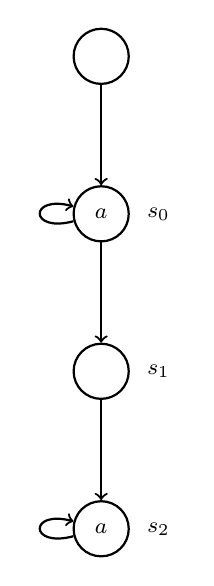
\begin{tikzpicture}[->,scale=1,label distance=0mm]
 \tikzstyle{every node}=[draw,shape=circle,minimum size=7mm,font=\footnotesize];
    \tikzstyle{every path}=[draw,thick];
    \node at (0, 2) (s) [label=right:$$] {$$};
    \node at (0, 0) (n0) [label=right:$s_0$] {$a$};
    \node at (0, -2) (n1) [label=right:$s_1$] {$$};
    \node at (0, -4) (n2) [label=right:$s_2$] {$a$};    
        \draw[->] (s) -- (n0);
    \draw[->] (n0) -- (n1);
    \draw[->] (n1) -- (n2);
		    
   \path[loop left] (n0) to (n0);
   \path[loop left] (n2) to (n2);
\end{tikzpicture}


}
\end{minipage}
\end{center}

The Kripke structure models the correct behaviour for the LTL formulae, but not for the corresponding ACTL formulae.


